\documentclass[master.tex]{subfiles}
\begin{document}

\chapter{Specification}
\label{chap:specification}

In this chapter, we will the full detail of phometa.
\section{Overview}
mainly talk about phometa UI structure, grids, and keymap pane

\section{Repository}
structure of repository
\begin{itemize}
\item add new sub-package or module inside a package (using package pane)
\item load/save repository using textarea in home pane + also talk about stdlib
\item add/swap nodes inside module
\item dedicate view for each node (using package pane)
\end{itemize}

\section{Node Comment}
\section{Node Grammar}
\section{Root Term}


\section{Input method of a term (TODO: modify this)}

% When a term is created, it can be in one of this mode

% \subsection{Editable up to Grammars}
% On this mode, we have a absolute control over a term i.e.\ both of grammar and
% term content can be changed, when it is created it will look like this,

% \centerline{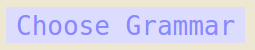
\includegraphics[scale=0.25]{term-input-method-001.png}}

% This is a completely blank term, we can set its grammar by clicking on it, then
% you will see option on keymap-pane (left-bottom corner of screen) as the following

% \centerline{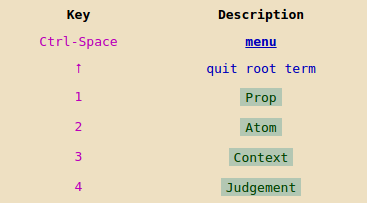
\includegraphics[scale=0.5]{term-input-method-002.png}}

% This show all of possible key-blinding including all of grammar that can be use,
% now we will select \pgmr{Prop} for this term's grammar by press \emph{1}
% (or alternatively clicking on \pgmr{Prop} directly), which now tern the
% term to be like this

% \centerline{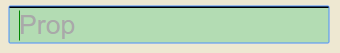
\includegraphics[scale=0.25]{term-input-method-003.png}}

% This means the term now know that it is \pgmr{Prop} term and hasn't know a
% content, and in order give a content we can set it to be either a construction
% term or meta-variable term. Now let make it a construction term, if you see
% keymap-pane again, it will look like this

% \centerline{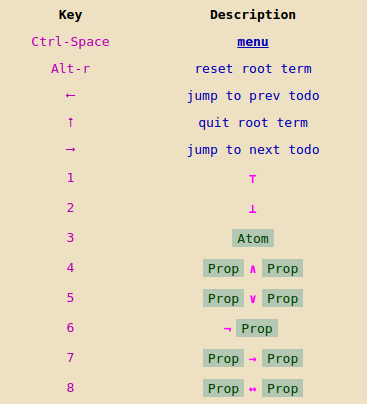
\includegraphics[scale=0.5]{term-input-method-004.png}}

% Similar to grammar selection, we can press the corresponded key-blinding that
% construct the term as we like. Let press \emph{7} for \bat{\pgmr{Prop}
%   \pifmt{$\rightarrow$} \pgmr{Prop}} and now the term become like this,

% \centerline{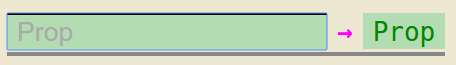
\includegraphics[scale=0.25]{term-input-method-005.png}}

% The root term now has \pifmt{$\rightarrow$} as the main connector and
% \emph{todos} spilt into two place, this process is recursive, you can try to
% split it again by e.g. press \emph{5} for \bat{\pgmr{Prop}
%   \pifmt{$\wedge$} \pgmr{Prop}} and get

% \centerline{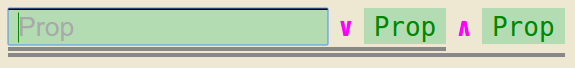
\includegraphics[scale=0.25]{term-input-method-006.png}}

% We also be able to move to other todos by clicking on target todo or simply
% press left arrow or right arrow for previous and next todo respectively.

% Next, we can make it to be meta-variable term by enter meta-variable name on the
% target todo then press enter. Let type \emph{A} for the first todo

% \centerline{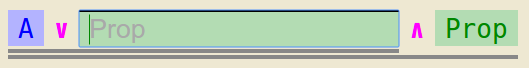
\includegraphics[scale=0.25]{term-input-method-007.png}}

% Now the first term become meta-variable and the cursor move to the next one
% automatically, please note that the meta-variable name must comply to \kVarRegex
% of corresponding grammar, otherwise, it will not convert to meta-variable. If
% you want to create an atom here, you can't just type directly since it is for
% \pgmr{Prop} meta-variable (As you can see from background text in todo),
% instead, you need to press \emph{3} to tell Phometa that it is construction for
% \pgmr{Atom}, like this

% \centerline{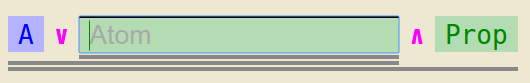
\includegraphics[scale=0.25]{term-input-method-008.png}}

% Now the background of current todo change from \emph{Prop} to \emph{Atom} and
% has extra underline so now you can type and atom

% \centerline{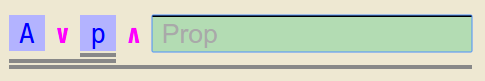
\includegraphics[scale=0.25]{term-input-method-009.png}}

% Not only meta-variable that can finish up todos, some of grammar choice just
% doesn't have sub-term, we could finish the last todo, by just press \emph{1} for \propTop

% \centerline{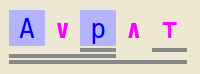
\includegraphics[scale=0.25]{term-input-method-010.png}}

% Now the term is finished, you can still return to the term and click some of
% them e.g.\ clicking \pvar{A}

% \centerline{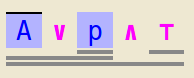
\includegraphics[scale=0.25]{term-input-method-011.png}}

% You can navigate to parent term my press up-arrow

% \centerline{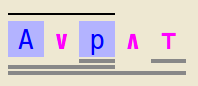
\includegraphics[scale=0.25]{term-input-method-012.png}}

% If you think you create some sub-term wrongly, you click on the that sub-term
% (in this is case \bat{\pvar{A} \propOr \bat{\pvar{p}}}) then press \emph{Alt-t}

% \centerline{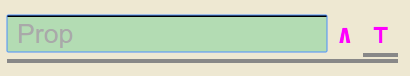
\includegraphics[scale=0.25]{term-input-method-013.png}}

% Or if everything is wrong including the root term grammar, you just press
% \emph{Alt-r}, this will go back to \emph{asking for grammar state}

% \centerline{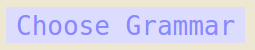
\includegraphics[scale=0.25]{term-input-method-001.png}}

% To give more example, let try to create \pgmr{Judgement} term, by click \emph{4}

% \centerline{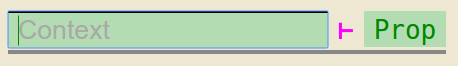
\includegraphics[scale=0.25]{term-input-method-014.png}}

% You might expect that after pressing \emph{4}, it should be just green area with
% background written as \emph{Judgement}, why it is auto expend like this, well,
% we have spacial case that if selecting grammar as just one choice and can't be
% meta-variable (we didn't state \kVarRegex\ for \pgmr{Judgement}), it will auto
% expend to that choice since that is the only action available.

% \subsection{Editable up to Term}
% This mode is the the same as editable up to grammar except that the grammar is
% given and we can't change it. If we try to reset the whole term \emph{Alt-r}, it
% the grammar still remain there.

% \subsection{Read only}
% In this mode, you can just view the term and nothing else.


\section{Node Rule}
\section{Node Theorem}

% \section{Placeholders}

% We will use placeholders to distinguish between different intention of string. The advantage of GUI-based theorem prover is that you can use any string that you like. No more reserve word or name clash. For example, we can use keyword as normal string as it will be label differently.

% \subsection{\pstr{string}} Represent newly created string, which is not linked from anywhere else before. This is useful when create a new identifier because we can't use a proper one as it doesn't exist before.

% \subsection{\pkw{keyword}} Keywords are built-in. We can't create a new keyword.

% \subsection{\pcomment{comment}} What ever you want to describe anything will be in this box.

% \subsection{\pid{identifier}} Show an identifier that has been selected in this module (i.e. the name referred to each node).

% \subsection{\pgmr{grammar}} The same as identifier but selection limited to grammar only. Grammar can be either inductive, literal, or sequence. For further information, see next section.

% \subsection{\pregex{regex}} Represent newly created regular expression (regex) pattern.

% \subsection{\pvar{variable}} Represent a (meta) variable used in rules and theorems. If there are variables that have the same name on the same root term, it is the same variable, this is useful in unification.

% \subsection{\plit{literal}} Represent literal inside a term which has literal grammar.

% \subsection{\pifmt{inductive formatter}} Sequent of symbol needed to construct inductive grammar.

% \subsection{\psfmt{sequence formatter}} Sequent of symbol needed to construct sequence grammar.

% \subsection{\pdfmt{definition formatter}} Sequent of symbol needed to construct definition.

% \subsection{\pdef{definition}} The same as identifier but limited to definition only.

% \subsection{\palias{alias}} The same as identifier but limited to alias only.

% \subsection{\prule{rule}} The same as identifier but limited to rule only.

% \subsection{\pthm{theorem}} The same as identifier but limited to theorem only.

% \subsection{\ppkgmod{package or module}} This is the result of selection of a list available in package or module. Please note that this is \textbf{not} a subset of identifier so so we can have package/module and identifier with the same name. But, on the same module, subpackage and module can't have the same name.

% \subsection{\bat{block \bat{\bat{as} term}}} We use underline to group (sub)term in to tree structure. This behaves similar to parenthesis, e.g. \bat{block \bat{\bat{as} term}} is in fact "(block (as (term)))" but looks a lot nicer. This is being used in
% \begin{itemize}
%     \item \bat{\ppkgmod{identify} \ppkgmod{module} \ppkgmod{path}}
%     \item \bat{\pgmr{inductive}  \pgmr{grammar} \pifmt{declaration}}
%     \item \bat{\pifmt{inductive} \pvar{term}}
%     \item \bat{\psfmt{sequence} \pvar{term}}
%     \item \bat{\pdfmt{definition} \pvar{term}}
% \end{itemize}

% \subsection{\bat{block as \bass{subsequence}}}
% When patten match on sequential term, sometime we want to express subsequence. but we can use just normal \bat{block as term} since it will be ambiguous to another thing. So we highlight subsequence with another color. E.g. \bat{\pvar{A} \psfmt{,} \bass{\pvar{B}} \psfmt{,} \pvar{C}}. \psfmt{,} So know exactly that \pvar{B} represent subsequence of this sequential term, not just another element. \\ \\

% TODO: write about term, root\_term, meta\_term, and hole.

% TODO: write about \textbf{input method} on term and meta\_term.

% TODO: write about \textbf{package explorer} which is the mechanism to dealing with \ppkgmod{packages} and \ppkgmod{modules} hierarchy.

% \newpage

% \section{Nodes and Attributes}

% At top level, will have a root package which consists of packages and modules

% each module is a collection of "nodes"

% there are several type of node as the following

% \begin{itemize}
%     \item \kOpen
%     \begin{itemize}
%         \item \kShowByDefault
%         \item \kHideByDefault
%     \end{itemize}
%     \item \kComment
%     \item \kGrammar
%     \begin{itemize}
%         \item \kInductive
%         \item \kLiteral
%         \item \kSequence
%         \item \kDictionary
%     \end{itemize}
%     \item \kDefinition
%     \item \kAlias
%     \item \kRule
%     \begin{itemize}
%         \item \kInference
%         \item \kCompound
%     \end{itemize}
%     \item \kTheorem
% \end{itemize}

% Note1. When we infer to "identifier", it can refer to any node since each node create new identifier except \kOpen and \kComment.

% Note3. Comment can be attribute of any node, if present, it must be the first attribute as well

% \subsection{\kOpen \bat{\ppkgmod{path} \ppkgmod{to} \ppkgmod{target module}} \{ \kShowByDefault \textbackslash \kHideByDefault \} }

% This is the way to import \pid{identifier} from another module to current module. Neither module name nor module path of this module will become identifier of current module (this is one of a reason why I use keyword "open" rather than "import"). The only result of this node is a set of identifier imported.

% \subsubsection{Common attributes}

% \begin{itemize}
%     \item \kRecursive \{\kTrue \textbackslash \kFalse\} \\
%     (Compulsory) If this is \kTrue, recursively import dependent identifiers which target module also use. In another word, transitive closure of dependent identifiers.
%     \item \kRename \pid{identifier from target module} \kTo \pstr{new\_name} \\
%     (Multiple) Import the target identifier and rename it as \pstr{new\_name}. Please note that this attribute is independent to show or hide by default.
%     \item \kInject \pid{injected node form current module} \kTo \pid{injectable node from target module} \\
% %   May be not necessary
% %     (Multiple) Inject dependency (from current module) to the copy of target module immediately before import that to current module.
% %     Please note that this does not effect the original target module. In fact, there is no way in phometa that allow dependent module to modify original one.
% %     We can only inject dependency to only the node which has attribute \kInjectable setted as \kTrue. This is nice since we can guarantee that the other node left untouched. Currently we have just \kInductive \kGrammar which allow \kInjectable attribute. But we might change it later.
% %     TODO: write an example involve injectable (i.e. first order logic which has pred different on context we are dealing with)
% \end{itemize}

% \subsubsection{\kShowByDefault and its attributes}
% For each identifier inside target module, if not state otherwise, do not import this to current module.
% \begin{itemize}
%     \item \kHide \pid{identifier from target module} \\
%     (Multiple) Tell phometa not to import this identifier. If \kRecursive is \kTrue this also work with the identifier that target module import as well.
% \end{itemize}

% \subsubsection{\kHideByDefault and its attributes}
% For each identifier inside target module, if not state otherwise, import this to current module.
% \begin{itemize}
%     \item \kShow \pid{identifier from target module} \\
%     (Multiple) The same effect as \kHide but show identifier instead of hiding it.
% \end{itemize}

% \subsection{node input method}

% We will give an example of \kOpen node alongside with the explanation, other nodes will be similar.

% Once the \kOpen node has been created (from module input method), user need to give path to target module (by module\_path input method) then they need to select (on the right corner of the header) weather this \kOpen node to be \kShowByDefault or \kHideByDefault.

% After that, the body of the node will be generated, all of "Compulsory" attributes (in this case, just \kRecursive) will be assign to default value. User can edit this by click "edit" on the right most of the header then user can,

% \begin{itemize}
%     \item enable/disable optional attributes (in this case, just \kComment)
%     \item add/remove/reorder multiple attributes
% \end{itemize}

% Please note that the order of attributes cannot change (except reordering in multiple attribute region).

% % This method is deprecate, but might be useful in the future.
% % \begin{itemize}[label={}]
% %     \item $\square$ \kComment
% %     \item $\oslash$ \kRecursive
% %     \item $\bigcirc$ show\_by\_default
% %     \begin{itemize}[label={}]
% %       \item $\oplus$ \kHide
% %     \end{itemize}
% %     \item $\bigcirc$ hide\_by\_default
% %     \begin{itemize}[label={}]
% %         \item $\oplus$ \kShow
% %     \end{itemize}
% %     \item $\oplus$ \kRename
% % \end{itemize}

% % \begin{itemize}
% %     \item $\oslash$ indicates that this attribute is compulsory, you can't add or delete it, it is there only for reference
% %     \item $\square$ indicates that this attribute is optional, you can toggle "tick box" to add or delete it
% %     \item $\bigcirc$ indicates that this attribute is selective, if you click circle, the attribute that you want will enable but also disable other (same level) circles
% %     \item $\oplus$ indicates that this attribute is multiple, you can click $\oplus$ to add new attribute, for reorder and delete individual you can do it directly in node body.
% % \end{itemize}

% \subsection{\kComment \pstr{summarise of comment, optional}}
% This is simply a node that we can use to short note. This is intended to be use as a way to describe or explain something involving multiple nodes. It is also use to explain module description.

% For detail of each individual node, there will be \kComment attribute of each node that node that you can use. See examples for further information.

% \subsection{\kGrammar \pstr{new grammar} \{\kInductive \textbackslash \kLiteral \textbackslash \kSequence \textbackslash \kDictionary\} }
% Introduce new grammar for this formal system

% \subsubsection{Common attributes}

% \begin{itemize}
%     \item \kVarRegex \pregex{regex} \\
%     (Optional) Patten of string that allow to be used as variable of this grammar. If this attribute is disabled, this grammar can't be in form of variable.
% \end{itemize}

% \subsubsection{\kInductive and its attributes}
% This is the standard way to define a grammar, an inductive term can be one of a form in \kChoice attributes. Then the subterm will be construct according to sub-grammar described in \kChoice
% \begin{itemize}
%     \item \kExtend \pgmr{inductive\_grammar} \\
%     (Optional) If present, it will import \kChoice from base grammar. Please note that the grammar used of this attributes must be inductive. Please note that derived grammar can be used everywhere that base grammar can.
%     \item \kChoice \bat{\pgmr{sequent} \pifmt{of} \pgmr{grammars} \pifmt{and formatter}} \kRef \pstr{reference} \\
%     (Multiple) One of the ways to instantiate this grammar. \pstr{reference} will be used in input method to refer back in to this choice. Please note that \pstr{reference} is in local name space of this inductive grammar
% \end{itemize}

%   TODO: On inductive term input method, when enter "construct by reference", if there is just one \kChoice then select it automatically.

% \subsubsection{\kLiteral and its attributes}
% This is another way to define grammar. When you want to define something like set of atom, numbers, etc. it is better to define this way. When you instantiate this kind of grammar, simply write a string, phometa will check it against \kRegex attribute.
% \begin{itemize}
%     \item \kRegex \pregex{regex} \\
%     (Compulsory) Pattern of string that allow to be used as literal of this grammar.
% \end{itemize}

% \subsubsection{\kSequence and its attributes}
% TODO: try to encode Sequence and Dictionary as Inductive grammar. Analogus to, encode tuple by dependent pair e.g. (a,b,c,d) => (a,(b,(c,d)))
% TODO: we will introduce spacial mechanism (perhaps built-in definition) to deal with sequence membership.
% This is a proper way to create collection like list, set, bag, etc. The grammar which is created in this way will get extra power from built-in rule which will become handy later.
% \begin{itemize}
%     \item \kSubGrammar \pgmr{grammar} \\
%     (Compulsory) Specify the grammar of elements of this sequence.
%     \item \kDelimiter \pstr{string} \\
%     (Optional) String to show as separator of each element. If this attribute doesn't exist. This sequence will not allow more than one element. Hence, become optional grammar (simialr to Maybe in Haskell and Option in OCaml)
%     \item \kWhenEmpty \pstr{string} \\
%     (Optional) String to show when the sequence is empty. If this attribute doesn't exist. This sequence cannot be empty which is useful for some particular sequence.
%     \item \kCommutative \{\kTrue or \kFalse\} \\
%     (Compulsory) State weather order is matter in this sequence or not. If \kTrue, there will be spacial rule which allow sequent to change order freely.
%     \item \kIdempotent \{\kTrue or \kFalse\} \\
%     (Compulsory) State weather elements are idempotent or not. If \kTrue, there will be spacial rule which allow sequent to remove or add some duplication on element.
% \end{itemize}

% \subsubsection{\kDictionary and its attributes}
% TODO: finish this and extend the entire phometa to support \kDictionary similarity to \kSequence

% TODO: we will introduce spacial mechanism (perhaps built-in definition) to deal with dictionary lookup/get\_keys/get\_values.

% This is a proper way to create lookup table. This structure might not look primitive but it is so common, so we decide to make it built-in.

% \begin{itemize}
%     \item \kKeyGrammar \pgmr{grammar} \\
%     (Compulsory) Specify the grammar of keys of this dictionary.
%     \item \kValueGrammar \pgmr{grammar} \\
%     (Compulsory) Specify the grammar of values of this dictionary.
%     \item \kSeparator \pstr{string} \\
%     (Compulsory) String to show as separator between key and value of each element of this dictionary.
%     \item \kDelimiter \pstr{string} \\
%     (Compulsory) String to show as separator of each element of this dictionary.
%     \item \kWhenEmpty \pstr{string} \\
%     (Compulsory) String to show when the sequence is empty.
% \end{itemize}

% \subsection{\kDefinition \pstr{new definition}}
% % TODO: finish this, please note that \kPartial is normal definition. But \kTotal in a definition that always be able to reduce (like total function), this can be achieved by not using \kMatch (use \kTotalMatch instead) and not call \kPartial \kDefinition.
% TODO: write an example involve \kLet ... \kBe
% % and \kTotal \kDefinition

% \subsection{\kAlias \pstr{new alias}}
% Alias is the similar to \kDefinition but has no parameter. It can to convert any matched (sub)term to the identifier of the alias (without built-in rule like in definition, just change the (sub)term directly by clicking on (sub)term underline). This is useful when dealing with a term which has a long subterm that is not necessary at the moment.
% % Whenever we said about definition (except \kDefinition node construction) we cover \kAlias as well.

% TODO: finish this

% \subsection{\kRule \pstr{new rule} \{\kInference \textbackslash \kCompound \} }
% TODO: finish this

% \subsection{\kTheorem \pstr{new theorem}}
% TODO: finish this

% \section{Available built-in rule so far}

% \subsection{\prule{sequence\_commutative}}
% Use this built-in rule to permute any sequential term that set \kCommutative as \kTrue.

% For input method, once user select to use this built-in rule, it will copy the original rule as premise then user can click on a delimiter on target sequence then the elements (including subsequences) that are adjacent to that delimiter will swap the position, keep swapping until we get the desired permutation. Once you are done click at built-in rule stop this interactive editing session.

% Please note that, this single command can permute several sequences at once.

% \subsection{\prule{sequence\_idempotent}}
% Use this built-in rule to duplicate or remove duplication on any sequential term. For input method, it is similar to \prule{sequence\_commutative} but user will click on element rather than delimiter (again, elements include subsequences as well, also if the element is \bat{block as term} then click its underline instead to avoid ambiguous on subterm)

% If the clicked element isn't the same previous element then duplicate the element, otherwise remove the element. By this mechanism, for any consecutive identical elements. We can keep duplicate by repeatly clicking the first term and keep remove duplication by repeatly clicking the second-term (or later terms)

% Stop this interactive editing session and ability to do on several sequences are the same as in \prule{sequence\_commutative}.

% \subsection{\prule{sequence\_commutative\_idempotent}}
% Can both permute and duplicate / remove duplicate like in \prule{sequence\_commutative} and \prule{sequence\_idempotent} in one go.


% \subsection{\prule{definition\_unfold}}
% Unfold target definitional term. For input method, once user select this build-in rule, user need to select one of definitional term (by clicking its underline), then it will unfold it.

% % Please note that, this method always work for \kTotal \kDefinition but might not be the case for \kPartial \kDefinition.

% \subsection{\prule{definition\_recursively\_unfold}}
% Similar to \prule{definition\_unfold} but will recursively attempt unfold further definitional terms on result of the first unfolding.

% Please note that, you can also select non-definitional term, then it will recursively unfold on definitional subterm of that term.

% \subsection{\prule{definition\_fold}}
% Fold target term. For input method, once user select this build-in rule, user need to select one of term then that term will become (term input method) hole, the user need to construct a term that can unfold to original term by one step.

% \subsection{\prule{definition\_recursively\_fold}}
% Similar to \prule{definition\_fold} but allow many step rather than just one step.

% TODO: write built-in rule for \kDictionary

\end{document}